\clearpage
\section{Thiết kế và hiện thực hệ thống}
\label{sec:implementation}

Chương~\ref{sec:model} đã mô tả Bloxorz như một bài toán tìm kiếm với trạng
thái, hành động và quy tắc chuyển rõ ràng. Từ mô hình đó, nhóm xây dựng chương
trình Python xoay quanh \texttt{GameEngine}. Thao tác của người chơi, bước tìm
kiếm của bộ giải và việc kiểm chứng lời giải đều tuân theo cùng một bộ luật. Nhờ
vậy, bốn thuật toán được đánh giá trên cùng một không gian trạng thái, còn giao
diện và công cụ đo đạc có thể phát triển độc lập với luật chơi.

\subsection{Kiến trúc tổng thể}

Hình~\ref{fig:system-architecture} cho thấy cách các thành phần phối hợp. Dữ
liệu màn chơi được \texttt{LevelLoader} kiểm tra trước khi tạo đối tượng
\texttt{Level}. \texttt{GameEngine} sử dụng các đối tượng dữ liệu về trạng thái,
hành động và luật nâng cao để xác định kết quả của mỗi nước đi. Giao diện dùng kết quả đó để
hiển thị và phát lại lời giải; các bộ giải dùng cùng bộ luật để tìm đường tới
đích; còn công cụ thực nghiệm ghi nhận kết quả chạy. Trong sơ đồ, mũi tên liền
biểu thị luồng xử lý hoặc dữ liệu, mũi tên nét đứt biểu thị việc dùng chung
\texttt{GameEngine}.

\begin{figure}[H]
\centering
\resizebox{0.98\textwidth}{!}{%
\begin{tikzpicture}[
    box/.style={draw=blue!65!black, rounded corners, fill=blue!6,
        text width=3.1cm, minimum height=0.9cm, align=center, font=\small},
    enginebox/.style={box, fill=green!13, draw=green!55!black},
    outbox/.style={box, fill=orange!10, draw=orange!70!black},
    flow/.style={-{Latex[length=2.1mm]}, thick},
    shared/.style={-{Latex[length=2mm]}, dashed, thick, draw=green!55!black}]
    \node[box] (json) at (0,0) {JSON màn chơi};
    \node[box] (loader) at (4.1,0) {LevelLoader\\kiểm tra dữ liệu};
    \node[box] (models) at (8.2,0) {Mô hình dữ liệu\\Level, State, Action};
    \node[enginebox] (engine) at (12.3,0) {GameEngine\\+ AdvancedRules};
    \draw[flow] (json) -- (loader);
    \draw[flow] (loader) -- (models);
    \draw[flow] (models) -- (engine);

    \node[box] (gui) at (0,-2.1) {GUI 3D\\nhập thao tác};
    \node[box] (controller) at (4.1,-2.1) {Controller\\trạng thái phiên chơi};
    \node[box] (worker) at (8.2,-2.1) {Luồng nền + hàng đợi\\giải tự động};
    \node[box] (manager) at (12.3,-2.1) {SolverManager\\BFS, DFS, UCS, A*};
    \draw[flow] (gui) -- (controller);
    \draw[flow] (controller) -- node[above, font=\scriptsize] {Solve} (worker);
    \draw[flow] (worker) -- (manager);
    \draw[shared] (engine) -- (manager);

    \node[outbox] (render) at (0,-4.2) {Dựng hình\\+ hoạt ảnh};
    \node[outbox] (replay) at (4.1,-4.2) {Phát lại\\chuỗi hành động};
    \node[outbox] (verifier) at (8.2,-4.2) {Kiểm chứng\\không qua giao diện};
    \node[outbox] (benchmark) at (12.3,-4.2) {Trình chạy thực nghiệm\\GameEngine mới mỗi lượt};
    \draw[flow] (controller) -- (render);
    \draw[flow] (controller) -- (replay);
    \draw[flow] (worker) -- (verifier);
    \draw[flow] (benchmark) -- (manager);
    \draw[shared] (engine.east) to[out=0,in=0,looseness=1.3] (benchmark.east);

    \node[outbox] (csv) at (10.25,-6.1) {CSV từng lượt/\\tổng hợp};
    \node[outbox] (charts) at (14.35,-6.1) {Biểu đồ};
    \draw[flow] (benchmark) -- (csv);
    \draw[flow] (csv) -- (charts);
    \node[font=\scriptsize, align=left, text width=6.5cm] at (3.55,-6.1)
        {Dùng chung GameEngine: chơi tay, bộ giải, kiểm chứng và thực nghiệm.\\
         Chơi tay: điều khiển $\rightarrow$ bộ luật $\rightarrow$ dựng hình.\\
         Giải: luồng nền $\rightarrow$ SolverManager $\rightarrow$ kiểm chứng $\rightarrow$ phát lại.};
\end{tikzpicture}%
}
\caption{Kiến trúc hệ thống và hai luồng tương tác; mọi thao tác hợp lệ được xác định bởi cùng GameEngine}
\label{fig:system-architecture}
\end{figure}

Khi chơi tay, bộ điều khiển gửi hành động tới \texttt{GameEngine} và hiển thị
kết quả sau hoạt ảnh. Khi giải tự động, bộ điều khiển lấy trạng thái tại thời
điểm bắt đầu giải; luồng nền gọi \texttt{SolverManager} từ trạng thái đó, kiểm
chứng lời giải rồi đưa kết quả vào hàng đợi. Bộ điều khiển chỉ phát lại lời
giải đã được xác minh. Công cụ thực nghiệm gọi bộ giải trực tiếp, không qua
giao diện hoặc luồng nền. Các nhánh cùng dùng \texttt{GameEngine} để sinh
trạng thái kế tiếp và kiểm tra điều kiện đích.

\subsection{Hiện thực mô hình và GameEngine}

Hệ thống đặt luật chơi trong \texttt{GameEngine} và dùng các đối tượng dữ liệu
bất biến để trao đổi thông tin giữa các thành phần. \texttt{models/level.py}
lưu lưới, vị trí đích, cầu và công tắc; \texttt{models/state.py} định nghĩa
\texttt{GameState} cùng hai dạng khối và mặt nạ cầu; \texttt{models/enums.py}
định nghĩa tư thế, hành động và loại công tắc. Tính bất biến cho phép dùng toàn
bộ trạng thái làm khóa của \texttt{dict}/\texttt{set}; hai trạng thái khác mặt
nạ cầu hoặc khối đang điều khiển không bị đồng nhất. \texttt{core/level\_loader.py}
đọc JSON, kiểm tra cấu trúc và tọa độ trước khi tạo đối tượng màn chơi. Cầu và
công tắc là dữ liệu bổ sung cho lưới ô.

\begin{table}[H]
\centering
\caption{Ánh xạ từ mô hình tìm kiếm sang hiện thực Python}
\label{tab:model-code-map}
\small
\begin{tabularx}{\textwidth}{@{}lX@{}}
\toprule
\textbf{Khái niệm} & \textbf{Hiện thực dùng chung} \\
\midrule
Level và luật tĩnh & \texttt{models/level.py}, \texttt{models/enums.py}, \texttt{core/level\_loader.py} \\
$S$ và $s_0$ & \texttt{models/state.py}; \texttt{GameEngine.get\_initial\_state()} \\
$A$ & Enum \texttt{Action} gồm bốn hướng và \texttt{SWITCH\_CUBE} \\
$T$ & \texttt{GameEngine.apply\_action()}, \texttt{get\_successors()} và \texttt{advanced\_rules.py} \\
$G$ & \texttt{GameEngine.is\_goal()} \\
$c$ & \texttt{solvers/costs.py: standard\_step\_cost()} \\
\bottomrule
\end{tabularx}
\end{table}

Mỗi hành động được \texttt{GameEngine} xử lý và trả về \texttt{TransitionResult}:
mã kết quả, trạng thái kế tiếp nếu có và sự kiện cho giao diện. Với nước đi di
chuyển, hệ thống tính vị trí mới, kiểm tra điều kiện nâng đỡ, xử lý hiệu ứng
công tắc, tách--ghép khối và cầu, rồi kiểm tra lại trước khi xét Goal
(Hình~\ref{fig:transition-pipeline}). Các quy tắc chi tiết nằm trong mô-đun
luật nâng cao; \texttt{GameEngine} quyết định thứ tự áp dụng. Riêng
\textsc{SwitchCube}, khi khối đã tách, chỉ đổi khối điều khiển mà không kích
hoạt lại công tắc hay thay đổi cầu. Bộ giải chỉ xét các bước chuyển
\texttt{APPLIED}/\texttt{WON}; nước đi không hợp lệ hoặc làm khối rơi không tạo
cạnh tìm kiếm.

\begin{figure}[H]
\centering
\begin{tikzpicture}[
    node distance=0.34cm,
    stage/.style={draw, rounded corners, fill=blue!7, minimum width=10.2cm,
        minimum height=0.65cm, align=center, font=\small},
    terminal/.style={draw, rounded corners, fill=green!12, minimum width=2.2cm,
        minimum height=0.6cm, align=center, font=\small},
    flow/.style={-{Latex[length=2mm]}, thick}]
    \node[stage] (input) {Nhận trạng thái $s$ và hành động $a$; kiểm tra dữ liệu};
    \node[stage, below=of input] (move) {Tính vị trí mới: lăn khối hoặc di chuyển khối đơn vị};
    \node[stage, below=of move] (support1) {Kiểm tra điều kiện nâng đỡ với trạng thái cầu hiện tại};
    \node[stage, below=of support1] (effect) {Phát hiện công tắc mới được nhấn; tách/ghép khối và đổi cầu};
    \node[stage, below=of effect] (support2) {Cập nhật mặt nạ cầu; kiểm tra điều kiện nâng đỡ lần cuối};
    \node[stage, below=of support2] (goal) {Kiểm tra Goal và tạo \texttt{TransitionResult}};
    \node[terminal, below left=0.48cm and 1.0cm of goal] (applied) {\texttt{APPLIED}};
    \node[terminal, below right=0.48cm and 1.0cm of goal] (won) {\texttt{WON}};
    \draw[flow] (input) -- (move);
    \draw[flow] (move) -- (support1);
    \draw[flow] (support1) -- (effect);
    \draw[flow] (effect) -- (support2);
    \draw[flow] (support2) -- (goal);
    \draw[flow] (goal) -- (applied);
    \draw[flow] (goal) -- (won);
\end{tikzpicture}
\caption{Thứ tự xử lý một hành động di chuyển trong GameEngine; nước đi rơi hoặc không hợp lệ dừng sớm}
\label{fig:transition-pipeline}
\end{figure}

\subsection{Kiến trúc hệ thống giải tự động}

\texttt{SolverManager} chọn một trong bốn bộ giải rồi gọi phương thức
\texttt{solve} với \texttt{GameEngine}, trạng thái đầu và các tùy chọn. Khi
người dùng yêu cầu giải từ giao diện, lời gọi này chạy trong luồng nền;
\texttt{SolverManager} không tự tạo luồng. \texttt{SearchOptions} cho phép cấu
hình hủy tìm kiếm, giới hạn thời gian, giới hạn số nút hoặc truyền hàm chi phí
và heuristic tùy chỉnh. Trong thực nghiệm, bốn bộ giải cùng sinh trạng thái kế
tiếp và kiểm tra đích qua \texttt{GameEngine}. Cách quản lý tập chờ xét, thứ
tự ưu tiên và điều kiện cập nhật chi phí là phần riêng của từng thuật toán ở
Chương~\ref{sec:algorithms}.

Khi tìm thấy Goal, \texttt{SolutionResult} chứa dãy hành động và
\texttt{SearchMetrics}: thời gian tìm kiếm, bộ nhớ cấp phát đỉnh do Python theo
dõi và số nút đã mở rộng. BFS/DFS lưu quan hệ cha--con để truy vết, UCS giữ
đường đi trong mỗi phần tử hàng đợi ưu tiên, còn A* dùng \texttt{came\_from}.
Kết quả phân biệt \texttt{solution\_length} (số hành động di chuyển),
\texttt{action\_count} (mọi hành động, kể cả đổi khối) và
\texttt{solution\_cost} (theo hàm chi phí của thuật toán). Với kết quả
\texttt{FOUND}, bộ kiểm chứng áp lại từng hành động qua \texttt{GameEngine},
yêu cầu mọi bước chuyển hợp lệ và trạng thái cuối thỏa điều kiện đích. Bản thân
bộ giải không phát lại lời giải.

\subsection{Giao diện đồ họa và điều khiển}

GUI 3D dùng Ursina trên Panda3D~\cite{ursina83}. \texttt{gui/app.py} tạo màn
hình bắt đầu, bàn chơi và menu chọn BFS/DFS/UCS/A*. Bộ dựng hình hiển thị ô,
khối và hoạt ảnh theo trạng thái cùng các sự kiện của \texttt{GameEngine}.

\begin{figure}[H]
\centering
\begin{subfigure}[b]{0.57\textwidth}
    \centering
    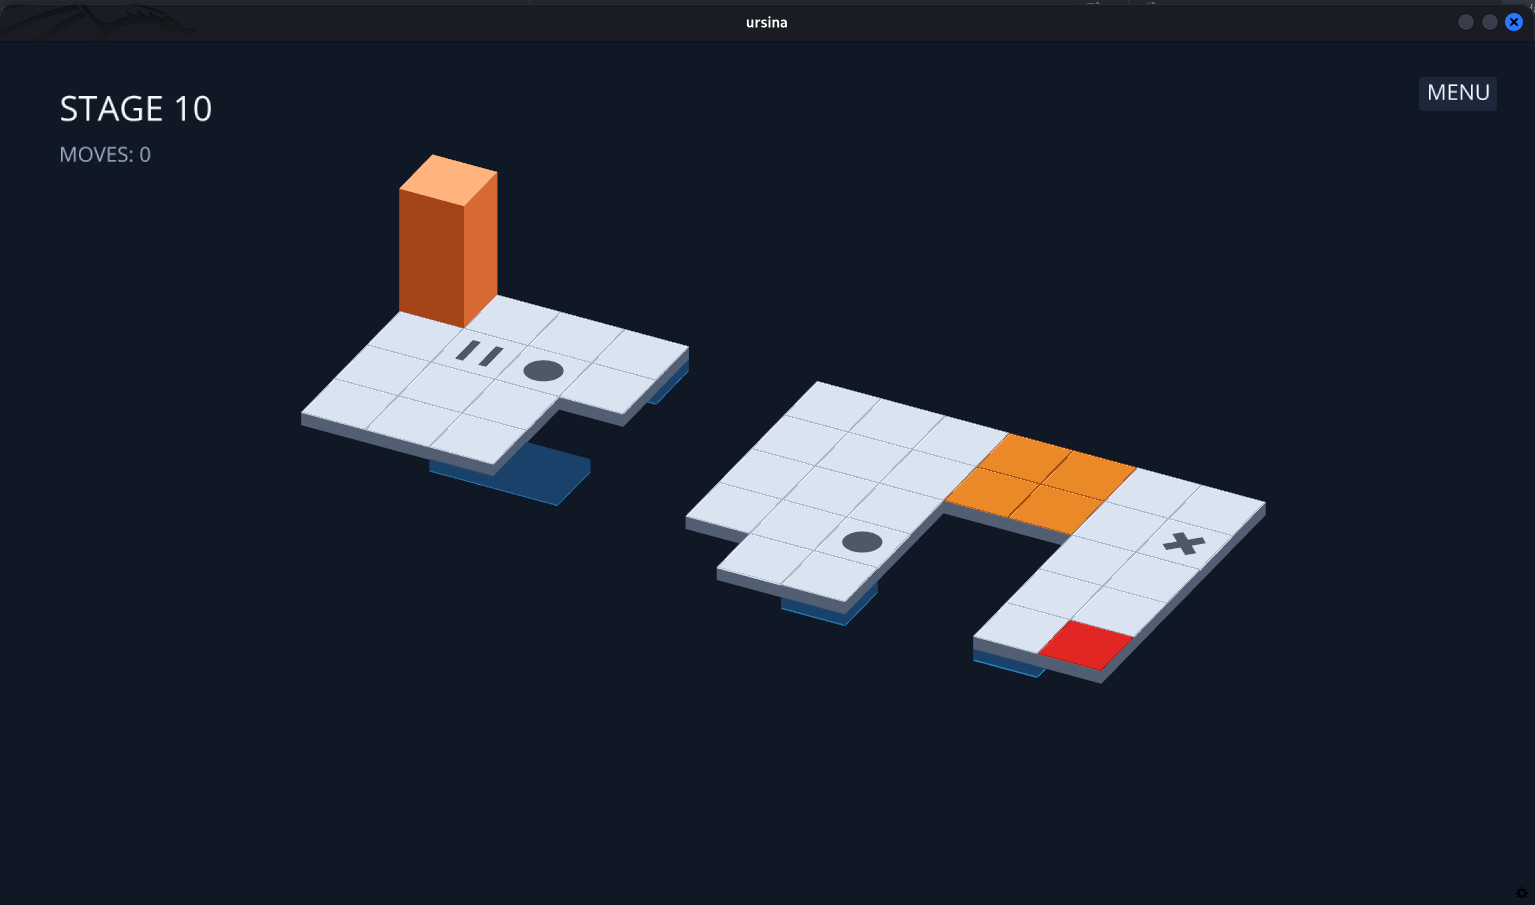
\includegraphics[width=\linewidth]{advanced_level.png}
    \caption{Màn chơi có công tắc, cầu, Fragile và Goal}
\end{subfigure}\hfill
\begin{subfigure}[b]{0.40\textwidth}
    \centering
    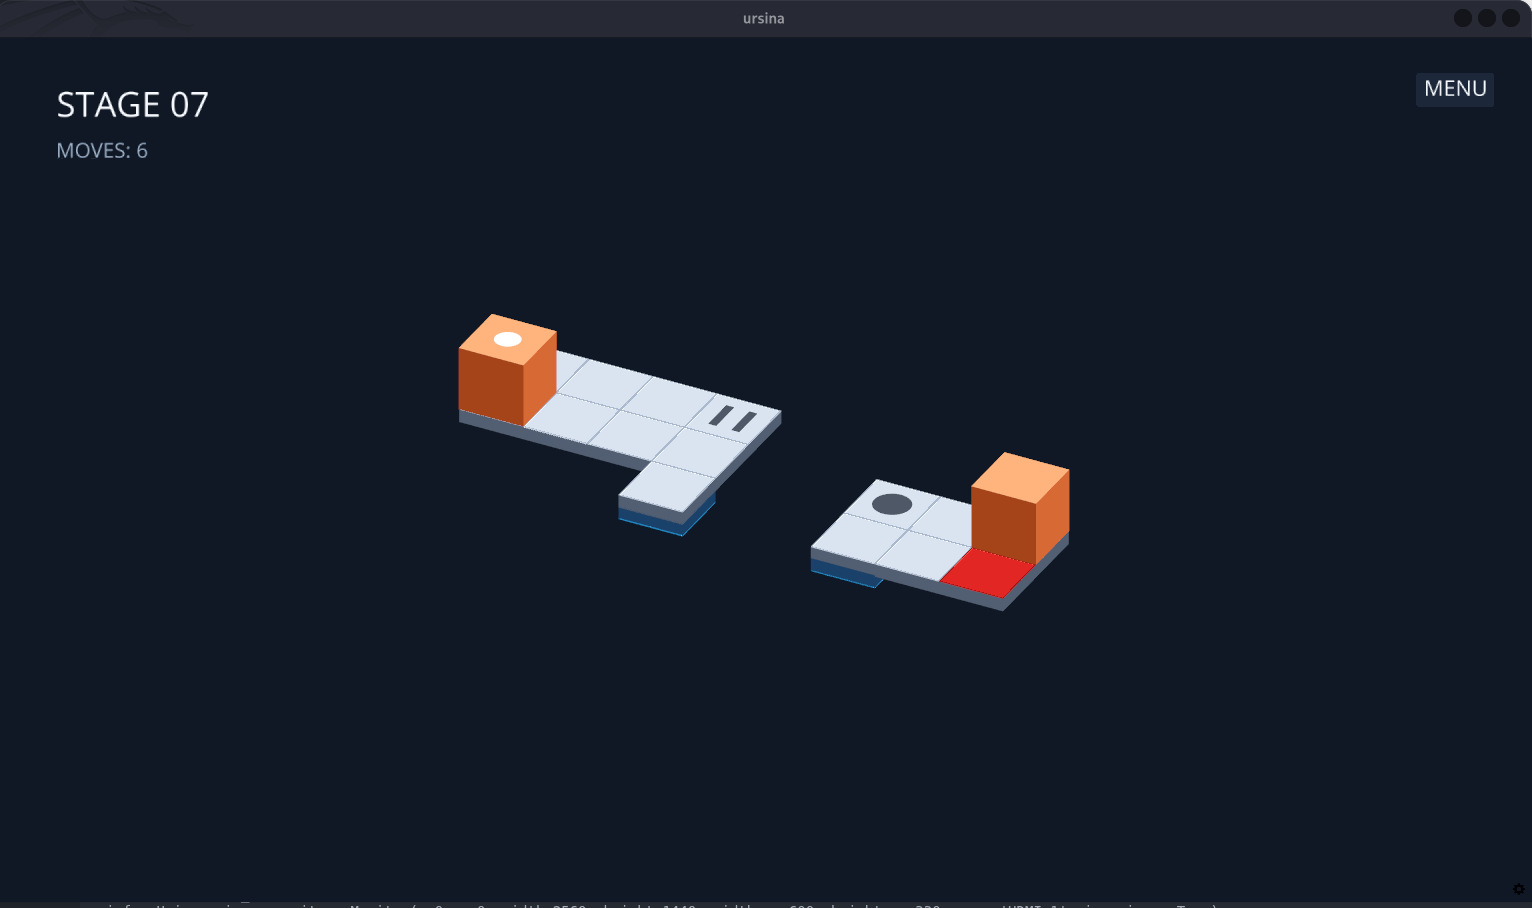
\includegraphics[width=\linewidth]{stage_07_split_blocks.png}
    \caption{Hai khối tách ở màn 07}
\end{subfigure}
\caption{Giao diện 3D minh họa các cơ chế nâng cao của Bloxorz Solver}
\label{fig:gui-mechanics}
\end{figure}

Bộ điều khiển giao diện quản lý trạng thái phiên chơi và phối hợp thao tác tay,
giải tự động cùng phát lại lời giải. Khi người chơi di chuyển, hành động được
xử lý qua \texttt{GameEngine}; trạng thái hiển thị chỉ cập nhật sau khi hoạt ảnh
kết thúc. New Game bắt đầu từ màn 01, Load Stage cho phép chọn màn khác, còn
Restart đưa màn hiện tại về trạng thái đầu.

Khi người chơi chọn thuật toán từ menu Solve, giao diện đưa màn hiện tại về
trạng thái đầu và giao trạng thái đó cho bộ giải chạy trên luồng nền. Luồng
nền kiểm chứng lời giải tìm được trước khi gửi kết quả qua hàng đợi về bộ
điều khiển. Mỗi yêu cầu giải có một mã riêng (\texttt{request\_id}); kết quả
cũ bị bỏ qua nếu người chơi hủy tìm kiếm, khởi động lại hoặc đổi màn. Với kết
quả \texttt{FOUND}, bộ phát lại thực hiện từng hành động qua cùng
\texttt{GameEngine} và đồng bộ với hoạt ảnh. Trong khi hoạt ảnh hoặc phát lại
đang chạy, giao diện không nhận thêm thao tác di chuyển tay.

\subsection{Đo hiệu năng và xác minh kết quả}

Công cụ thực nghiệm chạy các bộ giải trực tiếp, không qua giao diện. Mỗi lượt
được thực hiện trên một \texttt{GameEngine} mới và ghi kết quả vào CSV. Thời gian
tìm kiếm được đo bằng \texttt{perf\_counter}; bộ nhớ đỉnh là lượng cấp phát Python
cao nhất do \texttt{tracemalloc} theo dõi~\cite{python314}. Thời gian tải màn chơi,
dựng hình, ghi CSV và phát lại không nằm trong phép đo.

Sau khi chạy, kết quả của các lượt tìm thấy lời giải được tổng hợp thành bảng
CSV và biểu đồ. Bộ kiểm chứng áp lại dãy hành động qua \texttt{GameEngine} để
xác nhận lời giải mà không cần mở giao diện. Tập lệnh kiểm tra báo cáo còn đối
chiếu dữ liệu CSV và giải lại 60 cặp màn chơi--thuật toán để kiểm tra độc lập.
Quy trình đo và kết quả được trình bày ở Chương~\ref{sec:experiment} và
Chương~\ref{sec:results}.
